\documentclass[tikz,border=8pt]{standalone}

\usepackage[T1]{fontenc}
\usepackage{lmodern}
\usepackage{amsmath,amssymb}
\usepackage{xcolor}
\usetikzlibrary{arrows.meta,positioning,fit,calc,backgrounds}

\definecolor{ktaBlue}{RGB}{224,238,255}
\definecolor{ktaGreen}{RGB}{228,246,235}
\definecolor{ktaAmber}{RGB}{255,245,220}
\definecolor{ktaGrey}{RGB}{247,247,247}
\definecolor{ktaLine}{RGB}{38,38,38}
\definecolor{ktaSoft}{RGB}{95,95,95}

\begin{document}

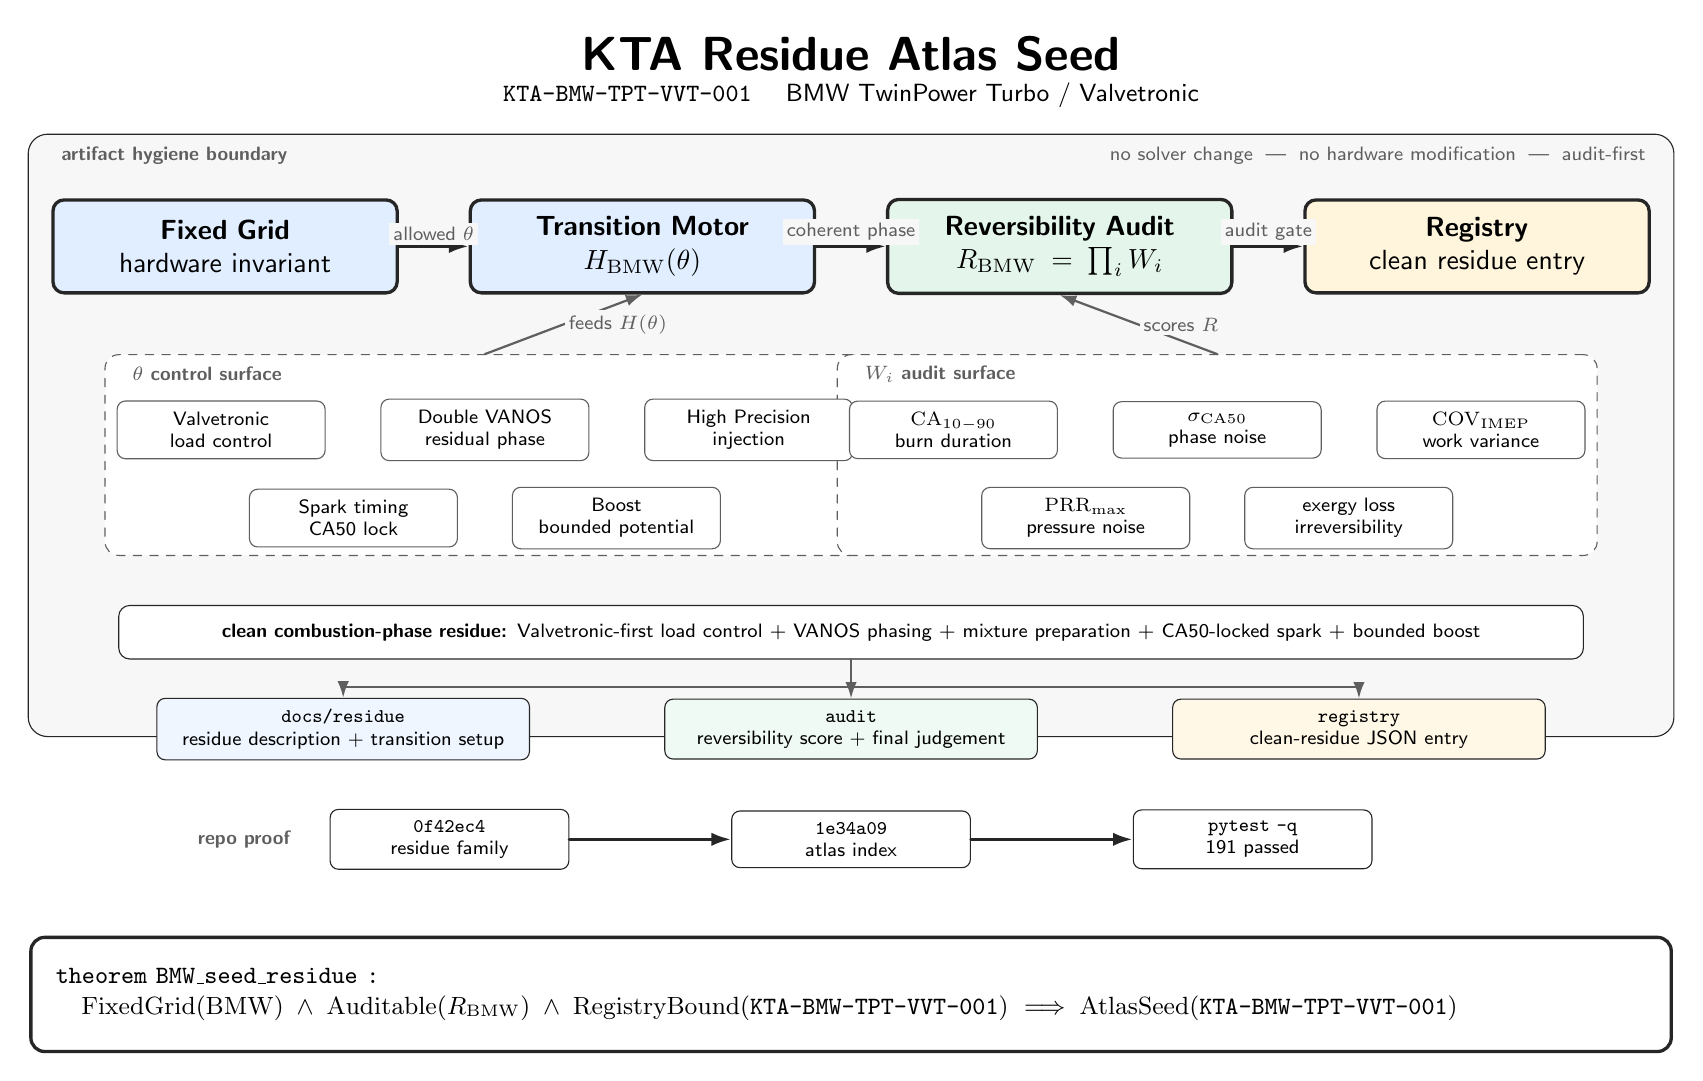
\begin{tikzpicture}[
  x=1cm,y=1cm,
  font=\sffamily,
  line cap=round,
  line join=round,
  >=Latex,
  core/.style={
    draw=ktaLine,
    rounded corners=4pt,
    fill=white,
    very thick,
    minimum width=4.20cm,
    minimum height=1.18cm,
    text width=3.95cm,
    align=center,
    inner sep=6pt
  },
  panel/.style={
    draw=ktaSoft,
    rounded corners=5pt,
    dashed,
    fill=white,
    minimum width=9.65cm,
    minimum height=2.55cm,
    align=center,
    inner sep=7pt
  },
  tag/.style={
    draw=ktaSoft,
    rounded corners=3pt,
    fill=white,
    minimum width=2.55cm,
    minimum height=0.62cm,
    text width=2.36cm,
    align=center,
    inner sep=4pt,
    font=\sffamily\scriptsize
  },
  repo/.style={
    draw=ktaLine,
    rounded corners=3pt,
    fill=white,
    minimum width=4.70cm,
    minimum height=0.68cm,
    text width=4.45cm,
    align=center,
    inner sep=4pt,
    font=\sffamily\scriptsize
  },
  commit/.style={
    draw=ktaLine,
    rounded corners=3pt,
    fill=white,
    minimum width=3.00cm,
    minimum height=0.72cm,
    text width=2.75cm,
    align=center,
    inner sep=4pt,
    font=\sffamily\scriptsize
  },
  arrow/.style={-{Latex[length=2.5mm,width=1.7mm]}, very thick, draw=ktaLine},
  softarrow/.style={-{Latex[length=2.1mm,width=1.45mm]}, thick, draw=ktaSoft},
  note/.style={font=\sffamily\scriptsize, align=center, text=ktaSoft, fill=ktaGrey, inner sep=1.5pt},
  label/.style={font=\sffamily\scriptsize\bfseries, align=center, text=ktaSoft}
]

% --------------------------------------------------------------------
% Header
% --------------------------------------------------------------------
\node[font=\sffamily\bfseries\LARGE, align=center] at (11.0,13.0)
  {KTA Residue Atlas Seed};
\node[font=\sffamily\small, align=center] at (11.0,12.47)
  {\texttt{KTA-BMW-TPT-VVT-001} \quad BMW TwinPower Turbo / Valvetronic};

% --------------------------------------------------------------------
% Artifact hygiene boundary
% --------------------------------------------------------------------
\node[
  draw=ktaLine,
  rounded corners=7pt,
  fill=ktaGrey,
  inner sep=0pt,
  minimum width=20.9cm,
  minimum height=7.65cm,
  anchor=center
] (boundary) at (11.0,8.15) {};

\node[anchor=west, label] at (0.85,11.70) {artifact hygiene boundary};
\node[anchor=east, note] at (21.15,11.70)
  {no solver change \;|\; no hardware modification \;|\; audit-first};

% --------------------------------------------------------------------
% Core flow
% --------------------------------------------------------------------
\node[core, fill=ktaBlue]  (grid)     at (3.05,10.55) {\textbf{Fixed Grid}\par hardware invariant};
\node[core, fill=ktaBlue]  (motor)    at (8.35,10.55) {\textbf{Transition Motor}\par $H_{\mathrm{BMW}}(\theta)$};
\node[core, fill=ktaGreen] (audit)    at (13.65,10.55) {\textbf{Reversibility Audit}\par $R_{\mathrm{BMW}}=\prod_i W_i$};
\node[core, fill=ktaAmber] (registry) at (18.95,10.55) {\textbf{Registry}\par clean residue entry};

\draw[arrow] (grid) -- node[above, note] {allowed $\theta$} (motor);
\draw[arrow] (motor) -- node[above, note] {coherent phase} (audit);
\draw[arrow] (audit) -- node[above, note] {audit gate} (registry);

% --------------------------------------------------------------------
% Panels: control surface and audit surface
% --------------------------------------------------------------------
\node[panel] (thetaPanel) at (6.35,7.90) {};
\node[panel] (auditPanel) at (15.65,7.90) {};

\node[label, anchor=west] at (1.75,8.93) {$\theta$ control surface};
\node[label, anchor=west] at (11.05,8.93) {$W_i$ audit surface};

% theta knobs, arranged in two rows
\node[tag] (valv)  at (3.00,8.22) {Valvetronic\par load control};
\node[tag] (vanos) at (6.35,8.22) {Double VANOS\par residual phase};
\node[tag] (inj)   at (9.70,8.22) {High Precision\par injection};
\node[tag] (spark) at (4.68,7.10) {Spark timing\par CA50 lock};
\node[tag] (boost) at (8.02,7.10) {Boost\par bounded potential};

% audit metrics, arranged in two rows
\node[tag] (ca)     at (12.30,8.22) {$\mathrm{CA}_{10-90}$\par burn duration};
\node[tag] (sigca)  at (15.65,8.22) {$\sigma_{\mathrm{CA50}}$\par phase noise};
\node[tag] (cov)    at (19.00,8.22) {$\mathrm{COV}_{\mathrm{IMEP}}$\par work variance};
\node[tag] (prr)    at (13.98,7.10) {$\mathrm{PRR}_{\max}$\par pressure noise};
\node[tag] (exergy) at (17.32,7.10) {exergy loss\par irreversibility};

\draw[softarrow] (thetaPanel.north) -- node[right, note] {feeds $H(\theta)$} (motor.south);
\draw[softarrow] (auditPanel.north) -- node[right, note] {scores $R$} (audit.south);

% --------------------------------------------------------------------
% Clean residue capsule
% --------------------------------------------------------------------
\node[
  draw=ktaLine,
  rounded corners=4pt,
  fill=white,
  minimum width=18.60cm,
  minimum height=0.68cm,
  text width=18.25cm,
  align=center,
  inner sep=5pt,
  font=\sffamily\scriptsize
] (capsule) at (11.0,5.65)
{\textbf{clean combustion-phase residue:} Valvetronic-first load control $+$ VANOS phasing $+$ mixture preparation $+$ CA50-locked spark $+$ bounded boost};

% --------------------------------------------------------------------
% Repository artifacts
% --------------------------------------------------------------------
\node[repo, fill=ktaBlue!52]  (docs) at (4.55,4.42) {\texttt{docs/residue}\par residue description + transition setup};
\node[repo, fill=ktaGreen!55] (audf) at (11.00,4.42) {\texttt{audit}\par reversibility score + final judgement};
\node[repo, fill=ktaAmber!70] (regf) at (17.45,4.42) {\texttt{registry}\par clean-residue JSON entry};

\draw[softarrow] (capsule.south) -- ++(0,-0.35) -| (docs.north);
\draw[softarrow] (capsule.south) -- (audf.north);
\draw[softarrow] (capsule.south) -- ++(0,-0.35) -| (regf.north);

% --------------------------------------------------------------------
% Provenance row
% --------------------------------------------------------------------
\node[label, anchor=east] at (4.00,3.02) {repo proof};
\node[commit] (c1) at (5.90,3.02) {\texttt{0f42ec4}\par residue family};
\node[commit] (c2) at (11.00,3.02) {\texttt{1e34a09}\par atlas index};
\node[commit] (c3) at (16.10,3.02) {\texttt{pytest -q}\par 191 passed};
\draw[arrow] (c1) -- (c2);
\draw[arrow] (c2) -- (c3);

% --------------------------------------------------------------------
% Mathlib-style theorem
% --------------------------------------------------------------------
\node[
  draw=ktaLine,
  rounded corners=5pt,
  fill=white,
  very thick,
  minimum width=20.8cm,
  minimum height=1.45cm,
  text width=20.2cm,
  align=left,
  inner sep=9pt,
  font=\sffamily\small
] (thm) at (11.0,1.05)
{\texttt{theorem BMW\_seed\_residue :}\par
$\quad \mathrm{FixedGrid}(\mathrm{BMW})\;\land\;\mathrm{Auditable}(R_{\mathrm{BMW}})\;\land\;\mathrm{RegistryBound}(\texttt{KTA-BMW-TPT-VVT-001})$
$\;\Longrightarrow\;\mathrm{AtlasSeed}(\texttt{KTA-BMW-TPT-VVT-001})$};

\end{tikzpicture}

\end{document}
